\setAuthor{Tundmatu autor}
\setRound{lahtine}
\setYear{2006}
\setNumber{G 2}
\setDifficulty{4}
\setTopic{Elektriahelad}

\prob{Elektriskeem}
Leida laengud $q_1$, $q_2$ ja $q_3$ kõikidel skeemil toodud kondensaatoritel.

\begin{center}
	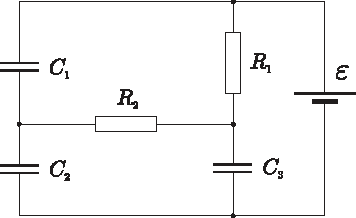
\includegraphics[width=0.7\linewidth]{2006-lahg-02-yl}
\end{center}

\hint
Kuna süsteemi stabiilses olekus on kondensaatorite pinge konstantne ei läbi neid ka vool.

\solu
Kondensaatori $C_1$ plaadid on ühendatud läbi takistite $R_1$ ja $R_2$. Seepärast laeng selle kondensaatori plaatidel on $q_1 = 0$ (pärast seda, kui on lõppenud kondensaatorite $C_2$ ja $C_3$ laadimine). Kuna pärast kondensaatorite laadimist voolud skeemis ei kulge, pinged kondensaatoritel $C_2$ ja $C_3$ on võrdsed $\mathcal E$. Järelikult, $q_2 = C_2\mathcal E$ ja $q_3 = C_3\mathcal E$.
\probend